\documentclass[a4paper,10pt]{article}
\usepackage[utf8]{inputenc}
\usepackage{hyperref}
\usepackage{graphicx}
\usepackage{amssymb}
\usepackage{amsmath}
\usepackage[margin=0.7in]{geometry}

\title{Building a Granular Dataset of UK Companies}
\author{Alfred Holmes}


\date{September 2018}
\begin{document}
   \maketitle
   \begin{abstract}
   The UK government, through the Office for National Statistics and Companies House release detailed data on UK companies which can be combined to generate. We show that, using publicly available data, it is possible to track the location and assets of companies through time and using few assumptions assign branches, employees and turnover to these companies in such a way as to match the Office for National Statistics annual reports.
   \end{abstract}
   \section{Introduction}
   To use contemporary techniques to model the UK economy, a detailed granular dataset of UK companies is required. Ideally the dataset would contain the employment size and turnover evolution of each company, as well as the location and number of employees of individual branches through time. From this, one could test hypotheses about company location decisions, track the flow of employment and generate a detailed picture of the changes in the UK economy easily.
   \subsection{Definitions}
   These definitions are used constituently throughout this document, and provide clarity when describing subtly different entities.
   \begin{itemize}
 	\item Company - an entity registered on Companies House. In June 2017 there were 3.1 million registered companies in the UK. 
 	\item Enterprise - a business that is reported by ONS. We assume that an enterprise is a collection of companies. In 2017 the ONS reported 2.7 million enterprises.
 	\item Local Unit - a site where an enterprise operates, e.g. a branch of a large supermarket chain or the only location from which a small firm operates.
 	\item Local Authority - a connected area of land the UK governed by a council. At the time of writing, local authorities have a population of 170 000 people and 7 000 enterprises on average. There are 391 local authorities in the UK.
   \end{itemize}

   \section{Data}
   The UK government through Companies House and the Office for National statistics release detailed data. All data used in this study is provided through the Open Government License.
   \subsection{Companies House}
   Companies House is the public service responsible for incorporating and dissolving companies in the UK, as well as storing and releasing company data. They provide monthly snapshots of basic company information - names, registered office addresses, SIC codes - as well as all the online accounts that have been filed since 2008 and also provide an API where more detailed information - changes of address and people of significant control - can be accessed on a company by company basis.
   \subsubsection{Snapshots}
   The companies house snapshots are only available for the current month and only contain active companies and don't contain data on the history of each company. Luckily \href{http://webarchive.org}{webarchive.org} has archived approximately 1 snapshot per year, so this can be used to get low resolution historic data for companies. The 
   \subsubsection{Accounts}
   If a company files its accounts online then that account filing is available to download through the companies house \href{http://download.companieshouse.gov.uk/historicmonthlyaccountsdata.html}{accounts data product}. Some small businesses are exempt from filing accounts, but for 2012 xx \% of companies filed accounts with 75\% of those accounts containing the current assets of the company. This increases to xx \% and xx \% respectively for 2017.
   The files are given as one XML (or HTML) file per account file per company per year. The most effective way to read these files is to recursively see if there is a number between two tags and if there is pull the number, its title and date.
   \subsubsection{Companies House API}
   The Companies House API can be used to get detailed information about a company given its name or company number. The API has a request limit of 2 requests per second per API key, so to make one query per company for all companies registered since 2012 it would take 32 days. The service does allow multiple API keys to be registered which can speed up data acquisition. The API can be used to get all the filings for a particular company, with the exact dates of each.
   \subsection{Office for National Statistics}
   The Office for National Statistics releases yearly summery datasets
   \subsubsection{Business Activity, Size and Location}
   \subsubsection{Other Useful Data}
   \paragraph{Population}
   \paragraph{Employment}

   \section{The Log Normal Hypothesis}
   To make the ONS data usable some sort of size distribution needs to be assumed. Using Maximum Likelihood Estimation (MLE) and the size bins, it is possible to fit distributions to the data. This has two benefits in that it assigns the mass of the probability distribution in a band in a sensible way and also removes the irritating \emph{250+} size band.
   \subsection{MLE and it's Bias}
  

   \begin{figure}
      \caption{Mean Bias Plane}
      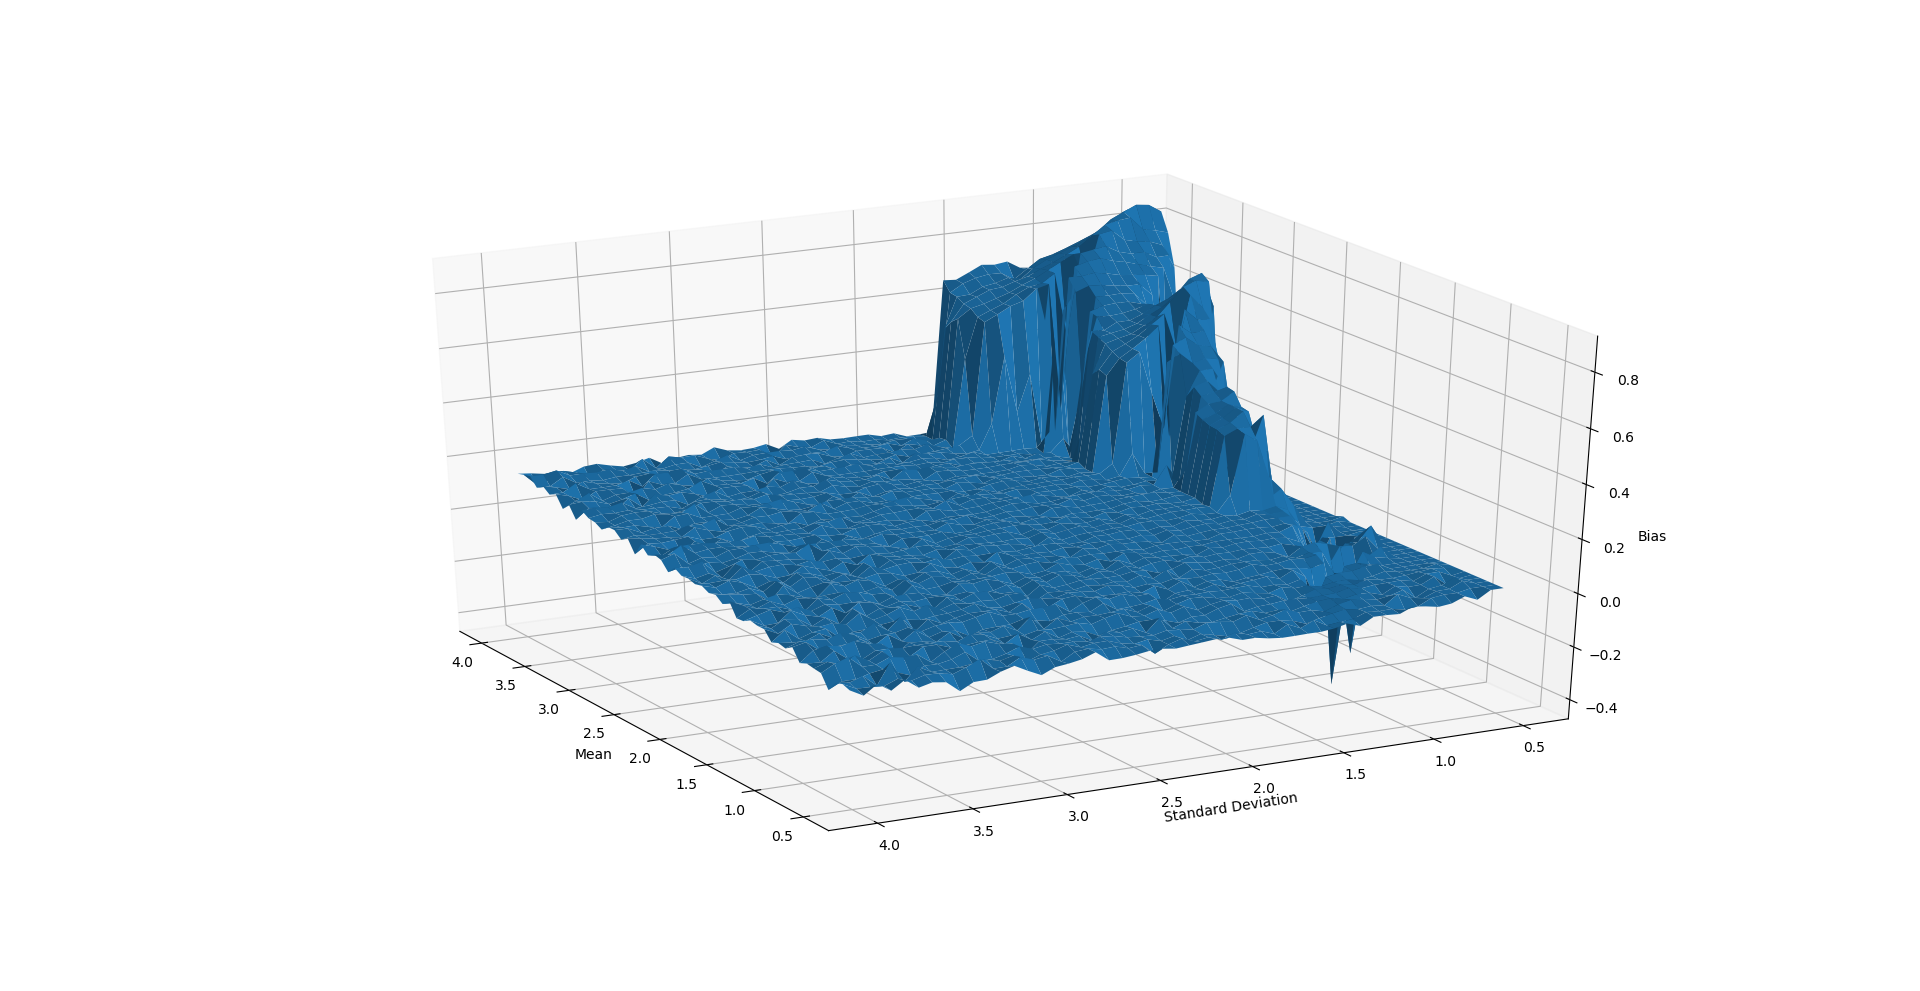
\includegraphics[width=\textwidth]{mean_bias_close}
      \label{fig:bias}
   \end{figure} 

   Assuming a log normal distribution where the size X of a company is such that $\log X \sim \mathcal{N}(\mu, \sigma^2)$, $\mu$ and $\sigma$ can be calculated by maximising the log likelihood, given by
   \begin{equation}
   l(\mu, \sigma) = \sum_i n_i \log \left( \Phi \left( \frac{\log a_{i + 1} - \mu}{\sigma} \right) - \Phi \left( \frac{\log a_{i} - \mu}{\sigma} \right) \right)
   \end{equation}
   since $\mathbb{P}(a_i < X < a_{i + 1}) = \mathbb{P}(\log a_i < \log X < \log a_{i + 1}) = \Phi \left( \frac{\log a_{i + 1} - \mu}{\sigma} \right) - \Phi \left( \frac{\log a_{i} - \mu}{\sigma} \right)$. \\
   Typically when dealing with bias from maximum likelihood estimates the bias depends on the number of observations in the sample and perhaps the values of the parameters themselves. Since the ONS data is binned and the sample size is large for each local authority, we assume that the sample proportions for each size band are the actual proportions for the distribution, to remove the dependence of the bias on the number of companies in the local authority. This can be justified by running simulations. We can then run simulations to examine the effects of the distribution parameters on the difference between the expected value of the MLE and the actual parameters. In doing so we find that for the region parameter space that we are interested in the bias forms a plane (see figure \ref{fig:bias}). The spikes in the bias are most likely formed by a poor match for the generated numbers and the size bands used in the ONS companies house report - so for example the whole sample is in one band.
   \\After simulating the parameter estimation, it is possible to fit parameters $(a, b, c)$ for $\mu$ and $\sigma$ to the observed bias plane such that, if $\hat{\mu}$ and $\hat{\sigma}$ are the MLE estimators
   \begin{align}
      a_1 \mu + b_1 \sigma + \mathbb{E}(\hat{\mu} - \mu) &= c_1\\
      a_2 \mu + b_2 \sigma + \mathbb{E}(\hat{\sigma} - \sigma) &= c_2
   \end{align}
   Now suppose that $\hat{\mu}'$ and $\hat{\sigma}'$ are unbiased estimators, this implies that
   \begin{align}
      c_1 - \mathbb{E}(\hat{\mu}) &= (a_1 - 1) \mathbb{E}(\hat{\mu}') + b_1 \mathbb{E}(\hat{\sigma}')\\
      c_2 - \mathbb{E}(\hat{\sigma}) &= a_2 \mathbb{E}(\hat{\mu}') + (b_2 - 1)\mathbb{E}(\hat{\sigma}')
   \end{align}
   If we define $\hat{\mu}'$ and $\hat{\sigma}'$ as
   \begin{align}
      \begin{pmatrix} \hat{\mu}' \\ \hat{\sigma}' \end{pmatrix}
      =
      \begin{pmatrix} a_1 - 1 & b_1 \\ a_2 & b_2 - 1 \end{pmatrix}^{-1}
      \begin{pmatrix} c_1 - \hat{\mu} \\ c_2 - \hat{\sigma} \end{pmatrix}
   \end{align}
   then the estimators are unbiased.





\end{document}